\PassOptionsToPackage{utf8}{inputenc}
\documentclass{bioinfo}
\usepackage{xspace}
\newcommand{\ie}{i.\,e.\@\xspace}
\newcommand{\wrt}{w.\,r.\,t.\@\xspace}
\newcommand{\dbb}[1]{{\color{blue}/******DBB:

#1

*********/
}}

\copyrightyear{2015} \pubyear{2015}

\access{Advance Access Publication Date: Day Month Year}
\appnotes{Original Paper}

\begin{document}
\firstpage{1}

\subtitle{Systems Biology}

\title[Robust disease module mining]{ROBUST: Robust disease module mining via enumeration of  price-collecting Steiner trees} 
\author[Bernett \textit{et~al}.]{%
Judith Bernett\,$^{\text{\sfb 1,}*}$, % 
Dominik Krupke\,$^{\text{\sfb 2,}*}$, % 
Sepideh Sadegh\,$^{\text{\sfb 1}}$, % 
Jan Baumbach\,$^{\text{\sfb 3,4}}$, % 
S\'andor P. Fekete\,$^{\text{\sfb 2}}$, % 
Tim Kacprowski\,$^{\text{\sfb 5,6}}$, % 
Markus List\,$^{\text{\sfb 1}}$, % 
and David B. Blumenthal\,$^{\text{\sfb 7,}\dagger}$}



\address{%
$^{\text{\sf 1}}$Chair of Experimental Bioinformatics, TUM School of Life Sciences, Technical University of Munich, Freising, Germany \\
$^{\text{\sf 2}}$Institute of Operating Systems and Computer Networks, Technical University of Brunswick, Brunswick, Germany\\
$^{\text{\sf 3}}$Chair of Computational Systems Biology, University of Hamburg, Hamburg, Germany\\
$^{\text{\sf 4}}$Department of Mathematics and Computer Science, University of Southern Denmark, Odense, Denmark\\
$^{\text{\sf 5}}$Division of Data Science in Biomedicine, Peter L. Reichertz Institute for Medical Informatics, Technical University of Brunswick and Hannover Medical School, Brunswick, Germany\\
$^{\text{\sf 6}}$Braunschweig Integrated Centre of Systems Biology (BRICS), Brunswick, Germany\\
$^{\text{\sf 7}}$Department Artificial Intelligence in Biomedical Engineering, Friedrich-Alexander University Erlangen-Nürnberg, Erlangen, Germany}

\corresp{%
$^\ast$Equally contributing first authors.\\
$^\dagger$To whom correspondence should be addressed.}

\history{Received on XXXXX; revised on XXXXX; accepted on XXXXX}

\editor{Associate Editor: XXXXXXX}

\abstract{\textbf{Motivation:} Disease module mining methods (DMMMs) mine molecular networks\,---\,usually, protein-protein interaction (PPI) networks\,---\,for subgraphs that constitute candidate disease mechanisms. Various DMMMs have been presented during the last years, using very different mathematical models. However, irrespectively of the employed models, most DMMMs share the problem that they include non-deterministic steps in their workflows, \ie, that the computed subnetworks vary when running the DMMMs multiple times on equivalent input. This lack of robustness has a negative effect on the trustworthiness of the obtained subnetworks and is hence detrimental for the wide-spread adoption of DMMMs in the biomedical sciences.\\
\textbf{Results:} To overcome this problem, we present a new DMMM called ROBUST (\textbf{robu}st disease module mining via enumeration of price-collection \textbf{S}teiner \textbf{t}rees). In a large-scale empirical evaluation, we show that, unlike all tested competitors, ROBUST achieves almost perfect robustness. Moreover, in most settings, ROBUST outperforms existing DMMMs in terms of functional relevance of the produced subgraphs, measured via KEGG gene set enrichment \wrt known disease-associated pathways and overlap with DisGeNet disease genes.\\
\textbf{Availability:} A Python 3 implementation and scripts to reproduce the results reported in this paper are available on GitHub: \href{https://github.com/bionetslab/robust}{https://github.com/bionetslab/robust}, \href{https://github.com/bionetslab/robust}{https://github.com/bionetslab/robust-eval}.\\
\textbf{Contact:} \href{mailto:david.b.blumenthal@fau.de}{david.b.blumenthal@fau.de}\\
\textbf{Supplementary information:} Supplementary data are available at \textit{Bioinformatics} online.}

\maketitle

\section{Introduction}

Over the last decades, high-throughput technologies and genome-wide association studies have generated an immense amount of omics data, enabling the generation of widely ramified and detailed interaction networks. Motivated by the possibility to uncover the pathobiology of complex diseases, the field of network medicine has emerged which tries to untangle these connections and pinpoint the source of certain clinical pictures. 
Because of the nature of the data, this field faces various challenges. Gene expression data is often noisy and protein-protein interaction (PPI) networks suffer from technical and literature bias, e.g. because proteins with known annotations tend to be the center of more interaction measurements and research questions. Because the node degree distribution of a PPI network follows a power law, mutations of healthy pathways typically have a cascading effect, leading to hundreds of differentially expressed genes. Additionally, not all of the genes triggering a certain disease might be differentially expressed in an experiment because the expression profiles are just a snapshot of the state of a cell. Therefore, the discovery of disease genes using simple statistical tests is unfeasible and algorithms exploiting the knowledge of PPI networks in combination with gene expression profiles are needed. 

Disease module mining methods (DMMMs)  try to identify significantly enriched subnetworks by projecting the expression data on the networks, applying different weight and scoring metrics to the network components and using various heuristics to find the modules, since the problem of finding a maximal-scoring connected subgraph is NP-hard (\cite{np_ideker2002}). Using these algorithms, subnetworks can be identified that are significantly associated with a certain disease, even when some of the individual nodes have a negligible score. These disease modules have successfully enabled new insights into complex diseases like Type-2 diabetes (\cite{diabetes_sharma2018, diabetes_fernandez2019}), pulmonary arterial hypertension (\cite{pulmonary_samokhin2018}), coronary heart disease (\cite{coronary_wang2018}) and asthma (\cite{asthma_sharma2015}).

%TODO: which algorithms to include?
Various algorithms have been proposed for identifying disease modules including DIAMOnD (\cite{diamond_ghiassian2015}), DOMINO (\cite{domino_levi2021}), MuST (multi-Steiner tree algorithm, \cite{covex_sadegh2020}), %from the DOMINO paper:
jActiveModules (\cite{np_ideker2002}), BioNet (\cite{bionet_beisser2010}), HotNet2 (\cite{hotnet2_leiserson2015}), NetBox (\cite{netbox_cerami2010}), KeyPathwayMiner (\cite{keypathwayminer_alcaraz2011, keypathway_baumbach2012, keypathwayminer_alcaraz2014, keypathwayminerweb_list2016}), %from the AMIM paper:
ClustEx2 (\cite{clustex2_ding2018}), COSINE (\cite{cosine_ma2011}), GiGA (\cite{giga_breitling2004}), GXNA (\cite{gnax_nacu2007}), GrandForest (\cite{grandforest_larsen2020}) and NetCore (\cite{netcore_barel2020}). Of these algorithms, DOMINO, DIAMOnD, MuST, ClustEx2 and NetBox require a binarized input (seed genes that were e.g. significant in the differential expression analysis) while the other methods project gene expression or mutation data on the PPI network. 

In their benchmark analysis, Levi \textit{et al.} have proven that most DMMMs learn mainly from network structure and not from the actual gene expression data. By permuting the gene expression measurements and comparing the resulting set of enriched GO terms with the set computed from the real activity scores, they showed that the overlap of the sets was high for most methods.  \cite{amim_lazareva2021} have additionally demonstrated that most DMMMs do not produce significantly more biologically meaningful disease modules when they are run on permuted networks that preserve the node degrees. An additional issue that has not been explicitly addressed yet, is the robustness of the methods. Most DMMMs include non-deterministic steps in their workflows, leading to variations in the resulting subnetworks when they are run multiple times on equivalent input. Furthermore, we hypothesized that the underlying heuristics are influenced by the order that the network was read into memory.  Because it is important to have a reliable output in order to achieve a widespread adoption of DMMMs in the biomedical research community, we present a new method, ROBUST, short for \textbf{robu}st disease module mining via enumeration of price-collection \textbf{S}teiner \textbf{t}rees. %TODO: High-level description of how ROBUST addresses this problem

We decided to compare our novel approach to DIAMOnD, DOMINO, MuST and a randomized version of MuST. Only methods with binary input were chosen since it was shown that they generally performed better because they were not as susceptible to noise (\cite{domino_levi2021}). DIAMOnD was selected since it is arguably the most widely used DMMM (\cite{diamond_popular_cui2019}). In the study by Lazareva \textit{et al}, DIAMOnD is outperformed by the recently introduced tool DOMINO. MuST and the randomized version of MuST (R-MuST) were included since they consitute the point of departure for the ROBUST method. %TODO more?    

In a large-scale empirical evaluation, we show that, unlike all tested competitors, ROBUST achieves almost perfect robustness. Moreover, in most settings, ROBUST outperforms  existing  DMMMs  in  terms  of  functional  relevance  of  the  produced  subgraphs, measured via KEGG gene set enrichment w. r. t. known disease-associated pathways and overlap with DisGeNet disease genes.


\dbb{Structure of the introduction should be as follows:
\begin{itemize}
\item General introduction to network medicine and disease module mining with some success stories. You can essentially rephrase what we've written in our BIB paper.
\item Overview of state-of-the-art methods with special focus on DOMINO, DIAMOnD, and MuST (as presented in CoVex). Reasoning for focussing on these DMMMs could be as follows: (1) In DOMINO paper, it's shown that DMMMs with binary input (\ie, seeds) typically perform better than those that project gene expression or mutation data on PPI networks. (2) Arguably, DIAMOnD is the most widely used DMMM with binary input. (3) DOMINO is the state-of-the-art tool, as shown in the original publication and in our BIB paper. (4) MuST constitutes the point of departure for the ROBUST method presented in this paper.
\item Introduction of the random bias/lack of robustness problem and motivation of its relevance (reliable output important for widespread adoption of DMMMs in biomedical research community).
\item High-level description of how ROBUST addresses this problem and very brief summary of most important results.
\end{itemize}
}

\section{Materials and Methods}

\subsection{Robust Optimization via Enumeration with Diversity}

\subsection{The Proposed Algorithm}

\subsection{Protocol and Data Used for Robustness Tests}

The methods were tested on a human PPI network obtained from the integrated interactions database (\cite{iid_kotlyar2019}) filtered based on experimental validation. The network therefore consists of 329,215 edges between 17,666 proteins. From this network, 903 small, unique seed sets were generated (2-20 seeds per set). Larger seed sets were not feasible since both MuST and R-MuST have high runtimes due to the computationally intensive Dijkstra computations. For more information about MuST and R-MuST, please refer to the Supplementary Information of \cite{covex_sadegh2020} and of this paper, respectively.  %TODO: how were they generated? -> Sepi 

In each iteration, the input network $G=(V,E)$ was permuted before running the respective algorithms. For each seed set $U \subseteq V$, this was repeated 20 times, yielding $(G_i)_{i=1}^{20}$. Let $M^{G_i} \subseteq V$ be the node set of a disease module for $(G_i,U)$ computed by any DMMM $ALG$. In order to evaluate the robustness of $ALG$, we compute the mean Jaccard index $r(ALG)$ as

\begin{equation}
    r(ALG) := \binom{n}{2}^{-1} \sum_{i=1}^{n-1} \sum_{j=i+1}^{n} \frac{|M^{G_i} \cap M^{G_j}|}{|M^{G_i} \cup M^{G_j}|} \in [0,1]
\end{equation}

Large values of $r(ALG)$ indicate that $ALG$ is robust to random storage order.

\subsection{Protocol and Data Used for Functional Relevance Tests}

Functional relevance tests were conducted by implementing custom wrappers for the AMIM test suite introduced by \cite{amim_lazareva2021}. In the test suite, gene expression datasets with case/control information for five complex diseases are used, namely amyotrophic lateral sclerosis (ALS), non-small cell lung cancer (LC), ulcerative colitis (UC), Chron's disease (CD) and Huntingtons disease (HD). The seed genes were obtained by applying a two-sided Mann-Whitney U-test on the case/control expression vectors and extracting all genes with a p-value smaller than $0.001/n$. Each set of seed genes was projected onto one of the five widely used PPI networks BioGRID (\cite{biogrid_oughtred2019}), APID (\cite{apid_alonso2016,apid_alonso2019}), STRING (\cite{string_szklarczyk2019}) with high confidence interactions only, HPRD (\cite{hprd_keshava2009}) and IID (\cite{iid_kotlyar2019}). Since we were only interested in the functional relevance results on the real dataset, none of the network generators of the test suite were used. 

Functional relevance was evaluated by computing gene set enrichment using the KEGG pathways (\cite{kegg_kanehisa2016}) corresponding to the diseases and by computing overlap coefficients with the disease-associated DisGeNET (\cite{disgenet_pinero2020}) gene sets. For more detailed information, please refer to \cite{amim_lazareva2021}.

\subsection{Protocol and Data Used for Case Study}

\section{Results}

\subsection{Effect of Hyper-Parameters on Robustness}

\subsection{Robustness in Comparison to Competitors}

\begin{figure*}[htb]
\centering
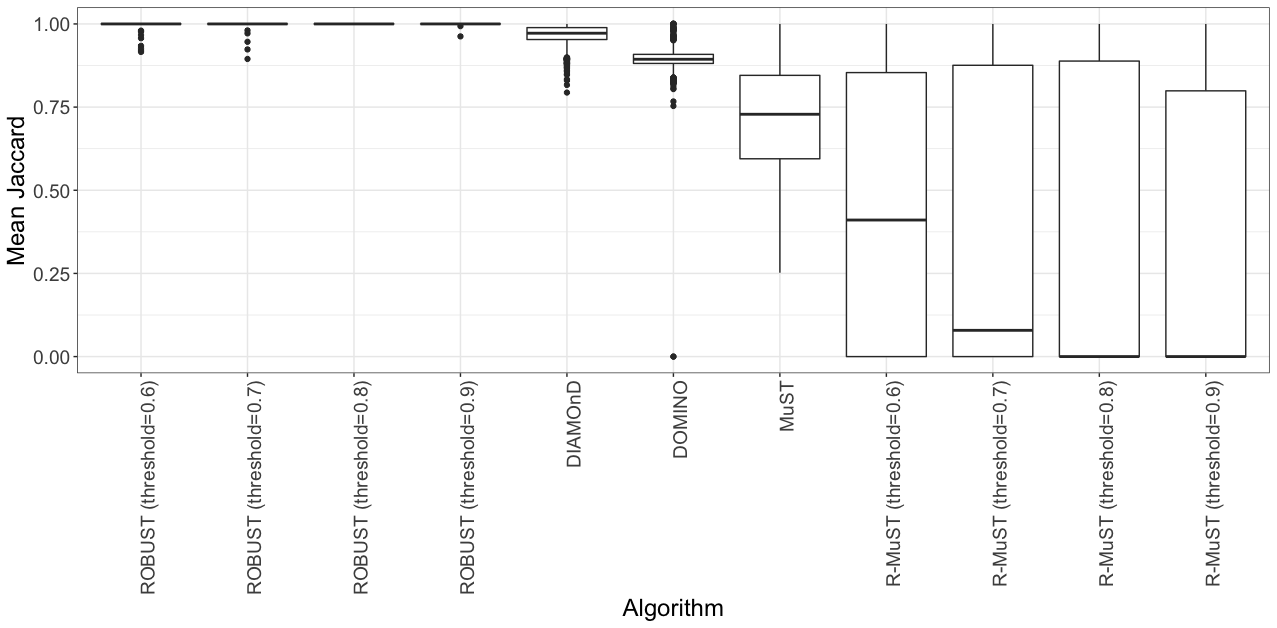
\includegraphics[width=0.95\linewidth]{img/robustness_results_ge05.png}
\caption[]{}
\label{robustness_subset}
\end{figure*}

%TODO: talk about thresholds and parameters
Figure \ref{robustness_subset} shows the distribution of the 903 mean Jaccard indices for each of the methods. It is clearly visible that the implementation of ROBUST is superior to its precursors MuST and R-MuST. In fact, the R-MuST results vary so strongly that we decided to leave the algorithm out when comparing functional relevance. DIAMOnD is more robust than DOMINO but ROBUST yields significantly higher mean jaccard indices than both methods (see Supplementary Table xxx) and achieves almost perfect robustness. 

\subsection{Functional Relevance in Comparison to Competitors}

\begin{figure*}[htb]
\centering
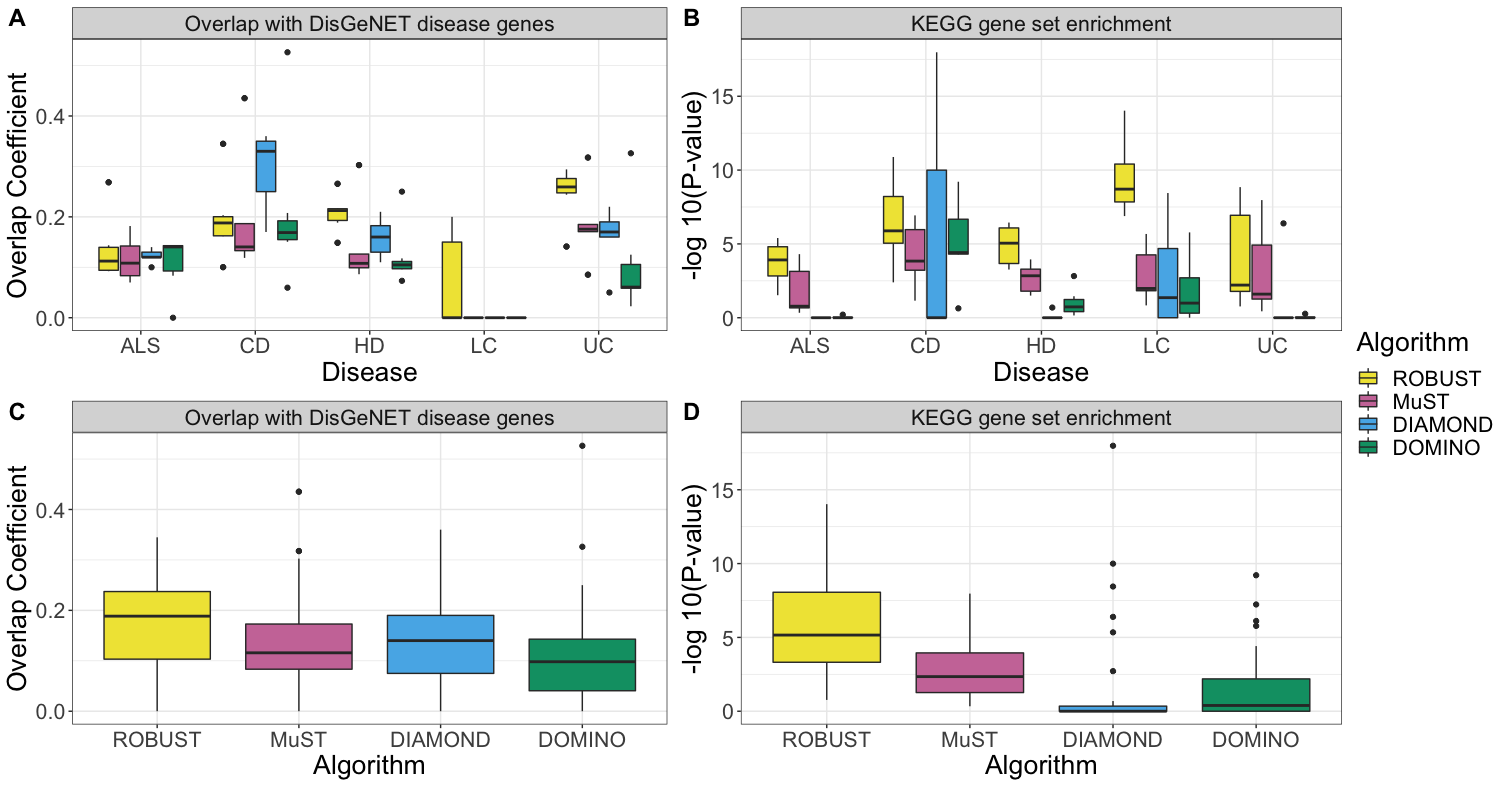
\includegraphics[width=0.95\linewidth]{img/functional_relevance_all.png}
\caption[]{}
\label{functional_relevance}
\end{figure*}


\subsection{Case Study: [NAME OF DISEASE]}

\section{Discussion}


\section*{Acknowledgements}


\section*{Funding}


\bibliographystyle{natbib}
\bibliography{references}
\end{document}
